\documentclass[slideopt,A4,showboxes,svgnames]{beamer}

%% list of packages here
\usepackage[absolute,showboxes,overlay]{textpos}
\usepackage{booktabs}
\usepackage{mathtools}
\usepackage{amsmath}
\usepackage{amssymb}
\usepackage{pifont}
\usepackage{multicol}
\usepackage{multirow}
\usepackage{array, makecell}
\usepackage{blkarray}
\usepackage[linesnumbered,ruled,vlined]{algorithm2e}
\usepackage[backend=biber, style=authoryear]{biblatex}
\renewcommand*{\nameyeardelim}{\addcomma\addspace}
\addbibresource{../references.bib}

\usepackage{theme/beamerthemeinria}


%%%%%%%%%%%%%%%%%%%%%%%%%%%%
% Paper dependent stuff    %
%%%%%%%%%%%%%%%%%%%%%%%%%%%%

\newcommand{\Tau}{\mathcal{T}}

%%%%%%%%%%%%%%%%%%%%%%%%%%%%
% Aesthetics               %
% over-underline, hat, bold%
%%%%%%%%%%%%%%%%%%%%%%%%%%%%

\newcommand{\eps}{\varepsilon}
\newcommand{\vareps}{\varepsilon}
\renewcommand{\epsilon}{\varepsilon}
%\renewcommand{\hat}{\widehat}
\renewcommand{\tilde}{\widetilde}
\renewcommand{\bar}{\overline}

\newcommand*{\MyDef}{\mathrm{\tiny def}}
\newcommand*{\eqdefU}{\ensuremath{\mathop{\overset{\MyDef}{=}}}}% Unscaled version
% \newcommand*{\eqdef}{\mathop{\overset{\MyDef}{\resizebox{\widthof{\eqdefU}}{\heightof{=}}{=}}}}
\newcommand{\eqdef}{\stackrel{def}{=}}


\def\:#1{\protect \ifmmode {\mathbf{#1}} \else {\textbf{#1}} \fi}
\newcommand{\CommaBin}{\mathbin{\raisebox{0.5ex}{,}}}

\newcommand{\wt}[1]{\widetilde{#1}}
\newcommand{\wh}[1]{\widehat{#1}}
\newcommand{\wo}[1]{\overline{#1}}
\newcommand{\wb}[1]{\overline{#1}}

% bf and bm missing due to conflict!!
\newcommand{\bsym}[1]{\mathbf{#1}}
\newcommand{\bzero}{\mathbf{0}}
\newcommand{\ba}{\mathbf{a}}
\newcommand{\bb}{\mathbf{b}}
\newcommand{\bc}{\mathbf{c}}
\newcommand{\bd}{\mathbf{d}}
\newcommand{\be}{\mathbf{e}}
\newcommand{\bg}{\mathbf{g}}
\newcommand{\bh}{\mathbf{h}}
\newcommand{\bi}{\mathbf{i}}
\newcommand{\bj}{\mathbf{j}}
\newcommand{\bk}{\mathbf{k}}
\newcommand{\bl}{\mathbf{l}}
\newcommand{\bn}{\mathbf{n}}
\newcommand{\bo}{\mathbf{o}}
\newcommand{\bp}{\mathbf{p}}
\newcommand{\bq}{\mathbf{q}}
\newcommand{\br}{\mathbf{r}}
\newcommand{\bs}{\mathbf{s}}
\newcommand{\bt}{\mathbf{t}}
\newcommand{\bu}{\mathbf{u}}
\newcommand{\bv}{\mathbf{v}}
\newcommand{\bw}{\mathbf{w}}
\newcommand{\bx}{\mathbf{x}}
\newcommand{\by}{\mathbf{y}}
\newcommand{\bz}{\mathbf{z}}

\newcommand{\bA}{\mathbf{A}}
\newcommand{\bB}{\mathbf{B}}
\newcommand{\bC}{\mathbf{C}}
\newcommand{\bD}{\mathbf{D}}
\newcommand{\bE}{\mathbf{E}}
\newcommand{\bF}{\mathbf{F}}
\newcommand{\bG}{\mathbf{G}}
\newcommand{\bH}{\mathbf{H}}
\newcommand{\bI}{\mathbf{I}}
\newcommand{\bJ}{\mathbf{J}}
\newcommand{\bK}{\mathbf{K}}
\newcommand{\bL}{\mathbf{L}}
\newcommand{\bM}{\mathbf{M}}
\newcommand{\bN}{\mathbf{N}}
\newcommand{\bO}{\mathbf{O}}
\newcommand{\bP}{\mathbf{P}}
\newcommand{\bQ}{\mathbf{Q}}
\newcommand{\bR}{\mathbf{R}}
\newcommand{\bS}{\mathbf{S}}
\newcommand{\bT}{\mathbf{T}}
\newcommand{\bU}{\mathbf{U}}
\newcommand{\bV}{\mathbf{V}}
\newcommand{\bW}{\mathbf{W}}
\newcommand{\bX}{\mathbf{X}}
\newcommand{\bY}{\mathbf{Y}}
\newcommand{\bZ}{\mathbf{Z}}

% calligraphic
\newcommand{\cf}{\mathcal{f}}
\newcommand{\cA}{\mathcal{A}}
\newcommand{\cB}{\mathcal{B}}
\newcommand{\cC}{\mathcal{C}}
\newcommand{\cD}{\mathcal{D}}
\newcommand{\cE}{\mathcal{E}}
\newcommand{\cF}{\mathcal{F}}
\newcommand{\cG}{\mathcal{G}}
\newcommand{\cH}{\mathcal{H}}
\newcommand{\cI}{\mathcal{I}}
\newcommand{\cJ}{\mathcal{J}}
\newcommand{\cK}{\mathcal{K}}
\newcommand{\cL}{\mathcal{L}}
\newcommand{\cM}{\mathcal{M}}
\newcommand{\cN}{\mathcal{N}}
\newcommand{\cO}{\mathcal{O}}
\newcommand{\cP}{\mathcal{P}}
\newcommand{\cQ}{\mathcal{Q}}
\newcommand{\cR}{\mathcal{R}}
\newcommand{\cS}{\mathcal{S}}
\newcommand{\cT}{\mathcal{T}}
\newcommand{\cU}{\mathcal{U}}
\newcommand{\cV}{\mathcal{V}}
\newcommand{\cW}{\mathcal{W}}
\newcommand{\cX}{\mathcal{X}}
\newcommand{\cY}{\mathcal{Y}}
\newcommand{\cZ}{\mathcal{Z}}

%%%%%%%%%%%%%%%%%%%%%%%%%%%%
% Math jargon              %
%%%%%%%%%%%%%%%%%%%%%%%%%%%%
\newcommand{\wrt}{w.r.t.\xspace}
\newcommand{\defeq}{\stackrel{\mathclap{\normalfont\mbox{\tiny def}}}{=}}
\newcommand{\maxund}[1]{\max\limits_{#1}}
\newcommand{\supund}[1]{\text{sup}\limits_{#1}}
\newcommand{\minund}[1]{\min\limits_{#1}}
\renewcommand{\epsilon}{\varepsilon}
\newcommand{\bigotime}{\mathcal{O}}


\DeclareMathOperator*{\argmin}{arg\,min} 
\DeclareMathOperator*{\argmax}{arg\,max} 
\DeclareMathOperator*{\cupdot}{\mathbin{\mathaccent\cdot\cup}}

%%%%%%%%%%%%%%%%%%%%%%%%%%%%
% Matrix operators         %
%%%%%%%%%%%%%%%%%%%%%%%%%%%%
\newcommand{\transpose}{^\mathsf{\scriptscriptstyle T}}
\newcommand{\transp}{\mathsf{\scriptscriptstyle T}}
\DeclareMathOperator{\Tr}{Tr}
\DeclarePairedDelimiterX{\inp}[2]{\langle}{\rangle}{#1, #2}

%%%%%%%%%%%%%%%%%%%%%%%%%%%%
% Statistic operators      %
%%%%%%%%%%%%%%%%%%%%%%%%%%%%
\newcommand{\probability}[1]{\mathbb{P}\left(#1\right)}
\newcommand{\probdist}{Pr}
\DeclareMathOperator*{\expectedvalue}{\mathbb{E}}
\DeclareMathOperator*{\variance}{\text{Var}}
\newcommand{\expectedvalueover}[1]{\expectedvalue\limits_{#1}}
\newcommand{\condbar}{\;\middle|\;}
\newcommand{\gaussdistr}{\mathcal{N}}
\newcommand{\uniformdistr}{\mathcal{U}}
\newcommand{\bernoullidist}{\mathcal{B}}

%%%%%%%%%%%%%%%%%%%%%%%%%%%%
% Algebraic Sets           %
%%%%%%%%%%%%%%%%%%%%%%%%%%%%
\newcommand{\Real}{\mathbb{R}}
\newcommand{\Natural}{\mathbb{N}}
\newcommand{\statespace}{\mathcal{X}}
\newcommand{\funcspace}{\mathcal{F}}
\newcommand{\dynaspace}{\mathcal{T}}


\newtheorem{theorem}{Theorem}
\newtheorem{definition}{Definition}
\newtheorem{lemma}{Lemma}
\newtheorem{proposition}{Proposition}
\providecommand*\propositionautorefname{Proposition}
\newtheorem{remark}{Remark}
\newtheorem{property}{Property}
\newtheorem{assumption}{Assumption}
\providecommand*\assumptionautorefname{Assumption}
\newtheorem{conjecture}{Conjecture}

\newtheorem*{definition*}{Definition}
\newtheorem*{theorem*}{Theorem}
\newtheorem*{proposition*}{Proposition}
\newtheorem*{remark*}{Remark}
\newtheorem*{example*}{Example}
\definecolor{darkspringgreen}{rgb}{0.09, 0.45, 0.27}
\definecolor{cadmiumgreen}{rgb}{0.0, 0.42, 0.24}
\newcommand{\hlr}[1]{\textcolor{Red}{#1}}
\newcommand{\hlb}[1]{\textcolor{Blue}{#1}}
\newcommand{\hlg}[1]{\textcolor{cadmiumgreen}{#1}}
\newcommand{\hlm}[1]{\textcolor{BurntOrange}{#1}}

\title[Robust-Adaptive Control]{Robust-Adaptive Control\\of Linear Systems:\\beyond Quadratic Costs}
\subtitle{Sous-titre}
\date[date]{date}
\author[Edouard Leurent]{\textbf{Edouard Leurent}\inst{1,2},\\
	Odalric-Ambrym Maillard\inst{1},\\
	Denis Efimov\inst{1}}
\institute{
	\inst{1} Univ. Lille, Inria, CNRS, \\ ~Centrale Lille, UMR 9189 – CRIStAL,\\
	\inst{2} Renault Group}

\begin{document}

\begin{frame}
    \titlepage
\end{frame}

\begin{frame}{Motivation}
Most RL algorithms rely on trial and {\red error}
\begin{itemize}
	\item {\blue random} exploration
	\item {\green optimism} in the face of uncertainty
\end{itemize}
\leavevmode\newline
Our work: ensure safety at all time
\begin{itemize}
	\item {\red pessimism} in the face of uncertainty
	\item {\green learn} from observations
\end{itemize}
\end{frame}

\begin{frame}{Setting}
\begin{alertblock}{Dynamical priors with structured uncertainty}
	State $x$, control $u$, bounded disturbance $\omega$
	\begin{align*}
	\dot{x}(t) &= {\orange A(\theta)}x(t) + B u(t) + \omega(t),\\
	{\orange A(\theta)} &= A + \sum_{i=1}^d {\orange \theta_i}\phi_i,
	\end{align*}
	where $A,B,\phi_1,\dots,\phi_d$ are \alert{known}.
\end{alertblock}

\begin{alertblock}{Performance measure}
	\begin{itemize}
		\item Discounted return $\sum_n\gamma^n R(x(t_n))$.
		\item Reward $R$ only assumed to be \alert{bounded}.
	\end{itemize}
\end{alertblock}
\end{frame}

\begin{frame}{Robust control framework}
Given $N$ observations,
\begin{enumerate}
	\item Build a {\red confidence region} for the dynamics
	$$\probability{{\orange \theta}\in {\red \cC_{N,\delta}}} \geq 1-\delta,$$
	\item Maximize the {\red worst-case} performance ${\red V^r}$
	$${\green\sup_{\bu\in{(\Real^q)}^\Natural}} \underbrace{{\red\inf_{\substack{\theta \in \cC_{N,\delta} \\ \omega\in[\underline{\omega},\overline{\omega}]^\Real}}} \left[\sum_{n=N+1}^\infty \gamma^n R(x(t_n))\middle| {\green \bu},{\red \theta},{\red\omega}\right]}_{{\red V^r(\bu)}},$$
\end{enumerate}

Related work
\begin{itemize}
	\item Robust Dynamic Programming (finite states only)
	\item Linear-Quadratic setting (quadratic costs only)
\end{itemize}
\end{frame}

\begin{frame}{Algorithm 1/3}
\begin{block}{Model Estimation}
	Confidence ellipsoid from non-asymptotic linear regression.
	\[\| \theta_{N,\lambda}  - \theta\|_{G_{N,\lambda}} \leq \beta_N(\delta) \]
\end{block}

\begin{center}
	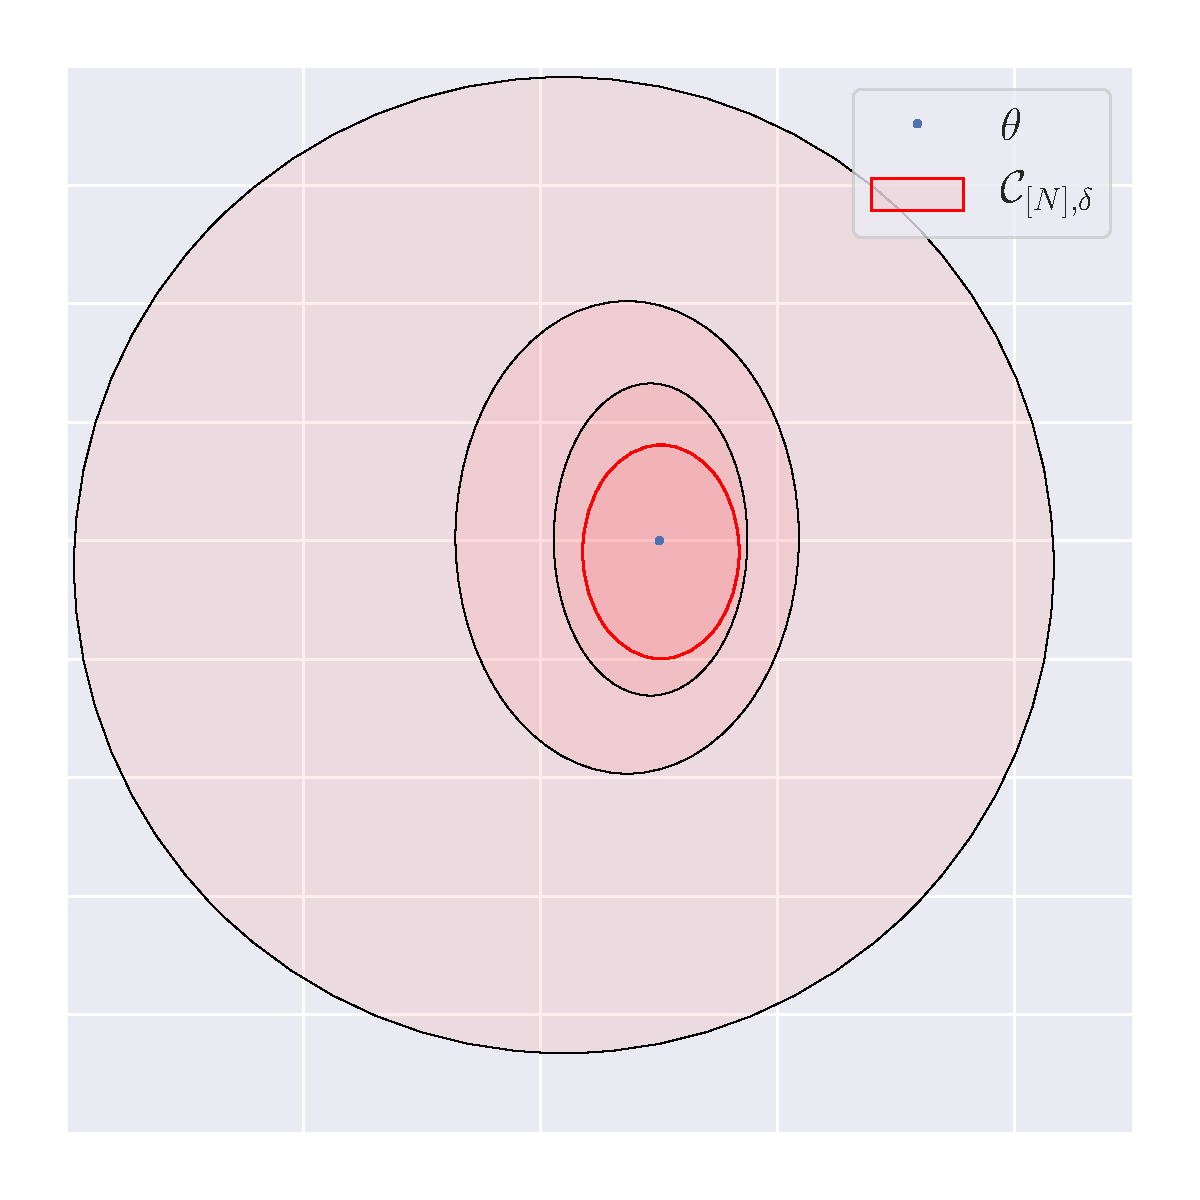
\includegraphics[width=0.4\linewidth]{../img/ellipsoid}
\end{center}

\end{frame}

\begin{frame}{Algorithm 2/3}
To optimise $V^r$ $\rightarrow$ approximate it by a tractable surrogate $\hat{V}^r$
\begin{block}{Interval Prediction} Propagate uncertainty ${\red \cC_{N,\delta}}$ through time and bound the state
	$${\blue \underline{x}(t)}\leq x(t)\leq{\blue \overline{x}(t)},\quad\forall t\geq t_N$$
\end{block}

\begin{center}
%	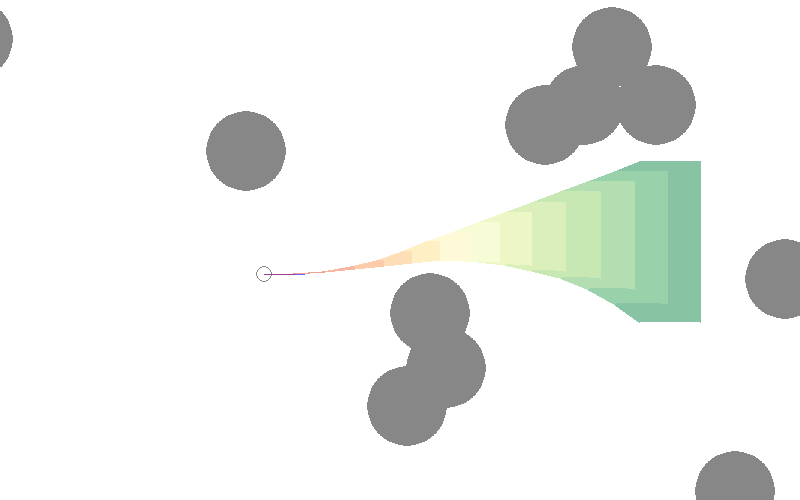
\includegraphics[width=0.6\linewidth]{../img/obstacle_small}
	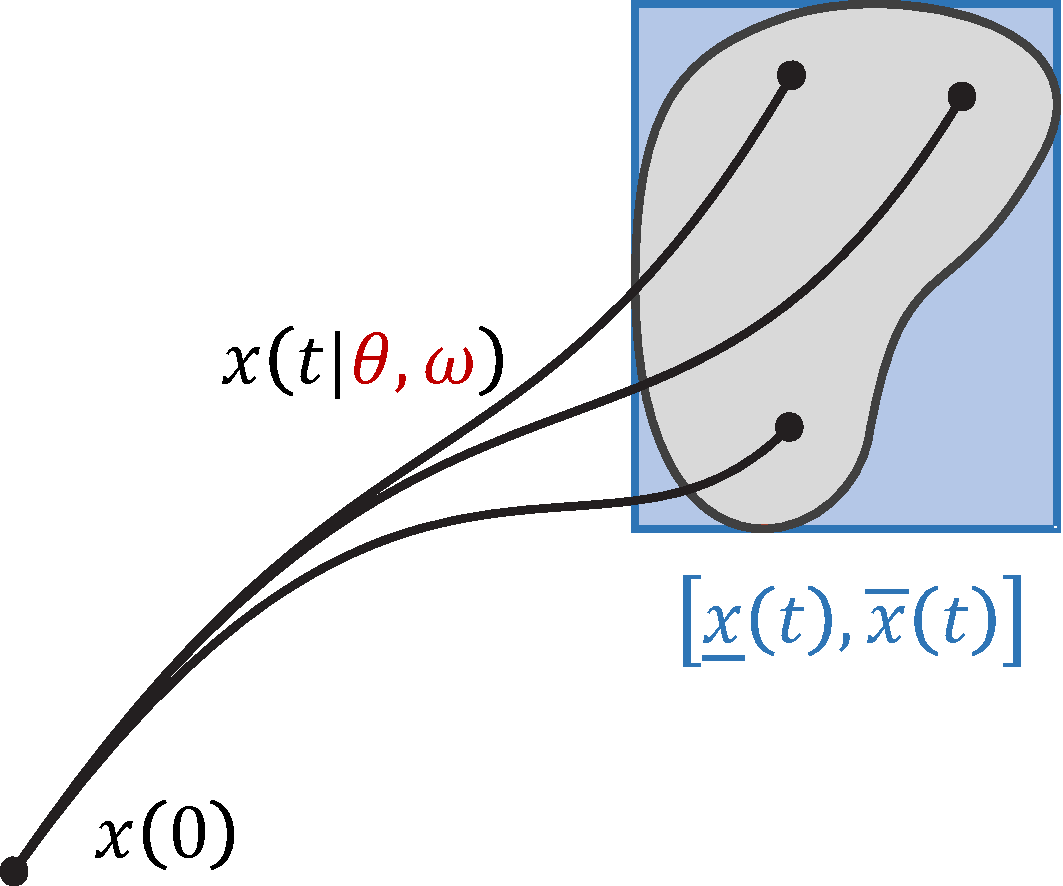
\includegraphics[width=0.4\linewidth]{./img/interval-hull}
\end{center}

\end{frame}

\begin{frame}{Algorithm 3/3}

\begin{block}{Pessimistic Planning}
	Surrogate pessimistic return, maximized by tree based-planning
	\[{\orange \hat{V}^r(\bu)} \eqdef \sum_{n=N+1}^\infty \gamma^n \min_{x\in{\blue [\underline{x}(t_n), \overline{x}(t_n)]}}  R(x).\]
\end{block}
\begin{center}
	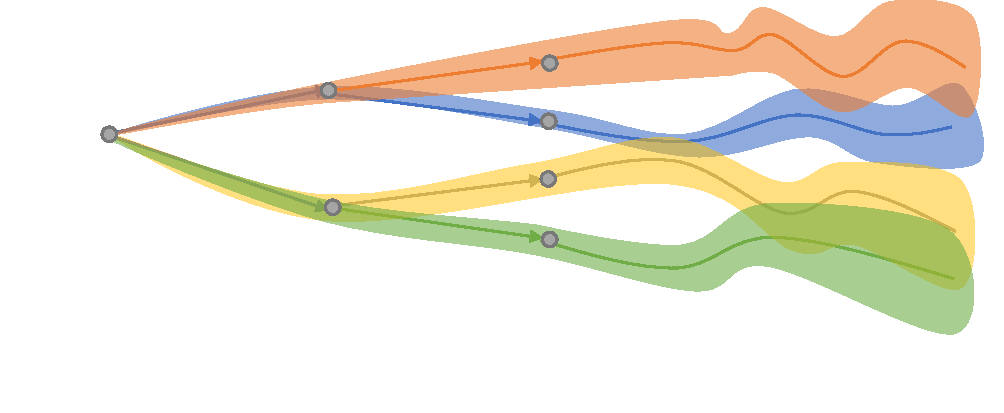
\includegraphics[trim={0 1.2cm 0 0}, clip, width=0.75\linewidth]{./img/planning}
\end{center}
\end{frame}

\begin{frame}{Results}
\begin{theorem}[Lower bound]
	\begin{equation*}
	{\orange \hat{V}^r(\bu)} \leq {\red V^r(\bu)} \leq V(u)
	\end{equation*}
\end{theorem}

\begin{theorem}[Suboptimality bound]
	Under two conditions:
	\begin{enumerate}
		\item Lipschitz rewards $R$:
		\item a stability condition over ${\red A(\theta_N)}$, for $N>N_0$
	\end{enumerate}
	we can bound the suboptimality with probability $1-\delta$ as:
	\begin{equation*}
	\underbrace{V(u_\star) - V(u_K)}_{\text{suboptimality}} \leq  {\red \underbrace{\Delta_\omega}_{\substack{\text{robustness to}\\ \text{disturbances}}}} + {\blue \underbrace{\cO\left(\frac{\beta_N(\delta)^2}{\lambda_{\min}(G_{N,\lambda})}\right)}_{\text{estimation error}}} + {\green \underbrace{\cO\left(K^{-\frac{\log 1/\gamma}{\log \kappa}}\right)}_{\text{planning error}}} 
	\end{equation*}
\end{theorem}
\end{frame}

\begin{frame}
\begin{corollary}[Asymptotic Near-Optimality]
	If the features $\phi_i x_n$ are \alert{persistently excited}, 
	\begin{itemize}
		\item the stability condition can be \alert{relaxed} to ${\orange A(\theta)}$ only
		\item the suboptimality bound takes the more explicit form
	\end{itemize}
	\begin{equation*}
	{V(u_\star) - V(u_K)}\leq  {\red \Delta_\omega} + {\blue {\cO\left(\frac{\log(N^{d/2}/\delta)}{N}\right)}} + {\green {\cO\left(K^{-\frac{\log 1/\gamma}{\log \kappa}}\right)}}
	\end{equation*}
	which ensures near-optimality as ${\blue N\to\infty}$ and ${\green K\to\infty}$.
\end{corollary}
\end{frame}

\begin{frame}{Experiments}

\end{frame}

\begin{frame}
\centering \LARGE Thank You!\\[1cm]
\large \emph{I am looking for a postdoctoral position.}
\end{frame}


\end{document}
